\section{Base di dati sistema anagrafe}

\subsection{Abstract}

L'obiettivo è sviluppare un servizio che tenga ordinati e renda sempre disponibili tutte le informazioni relative a nomi, gruppi, peculiarità di ognuno dei sensori, delle aree, e dei lampioni. 

Queste informazioni sono particolarmente utili per contestualizzare ognuna delle componenti {\it{hardware}} del sistema.

\subsection{Analisi dei requisiti}

\subsection{Progettazione concettuale}

\subsubsection{Analisi delle entità}

\textbf{Se non specificato l'attributo è NOT NULL}

%AREA
\begin{center}
    \begin{tabularx}{\textwidth}{|l|l|l|X|}
        \hline
        \rowcolor{gray!30}
        \multicolumn{4}{|c|}{\textbf{AREA}}\\
        \hline
        id & INTEGER & Identifica univocamente un'area all'interno del sistema & Chiave\\
        \hline
        nome & VARCHAR(50) & \multicolumn{2}{l|}{Il nome dell'area} \\
        \hline
        autoMode & BOOLEAN & \multicolumn{2}{l|}{Specifica se l'area viene gestita in modalità automatica o no (manuale)} \\
        \hline
        lvlInf & VARCHAR(50) & \multicolumn{2}{l|}{In area gestita in modalità automatica, questo è il livello di luminosità} \\ & & \multicolumn{2}{l|}{a cui vengono posti i lampioni se non vengono rilevate persone all'interno dell'area} \\
        \hline
        lvlSup & VARCHAR(20) & \multicolumn{2}{l|}{In area gestita in modalità automatica, questo è il livello di luminosità} \\ & & \multicolumn{2}{l|}{a cui vengono posti i lampioni se vengono rilevate persone all'interno dell'area} \\
        \hline
    \end{tabularx}
\end{center}

%MISURATORE
\begin{center}
    \begin{tabularx}{\textwidth}{|l|l|l|X|}
        \hline
        \rowcolor{gray!30}
        \multicolumn{4}{|c|}{\textbf{MISURATORE}}\\
        \hline
        id & SERIAL & Identifica univocamente un misuratore del livello di luminosità & Chiave\\
        \hline
        tipo & VARCHAR(10) & \multicolumn{2}{l|}{La tipologia del misuratore} \\
        \hline
        latitudine & REAL & \multicolumn{2}{l|}{Latitudine delle coordinate geografiche in cui viene posto il misuratore} \\
        \hline
        longitudine & REAL & \multicolumn{2}{l|}{Longitudine delle coordinate geografiche in cui viene posto il misuratore} \\
        \hline
        idArea & INTEGER & Identifica l'area a cui fa riferimento il misuratore & Chiave esterna: Area(id)\\
        \hline
    \end{tabularx}
\end{center}

%SENSORE
\begin{center}
    \begin{tabularx}{\textwidth}{|l|l|X}
        \hline
        \rowcolor{gray!30}
        \multicolumn{3}{|c|}{\textbf{SENSORE}}\\
        \hline
        raggio & INTEGER & Il raggio d'azione entro il quale il sensore è in grado di rilevare persone \\
        \hline
    \end{tabularx}
\end{center}

%LAMPIONE
\begin{center}
    \begin{tabularx}{\textwidth}{|l|l|X|}
        \hline
        \rowcolor{gray!30}
        \multicolumn{3}{|c|}{\textbf{LAMPIONE}}\\
        \hline
        wattaggio & INTEGER & Consumo energetico del lampione \\
        \hline
    \end{tabularx}
\end{center}

\subsubsection{Analisi delle relazioni e delle cardinalità}

\begin{itemize}

    \item Area - Misuratore: \textbf{Appartenenza}
    \begin{itemize}
        \item Un misuratore è contenuto in una ed una sola area (1,1);
        \item Un'area contiene da 0 a N misuratori (0,N);
    \end{itemize}
    
\end{itemize}

\subsubsection{Generalizzazioni}

\begin{itemize}
    \item Lampione è generalizzazione totale esclusiva di Misuratore;
    \item Sensore è generalizzazione totale esclusiva di Misuratore;
\end{itemize}

\subsubsection{Schema ER concettuale}

\begin{center}
    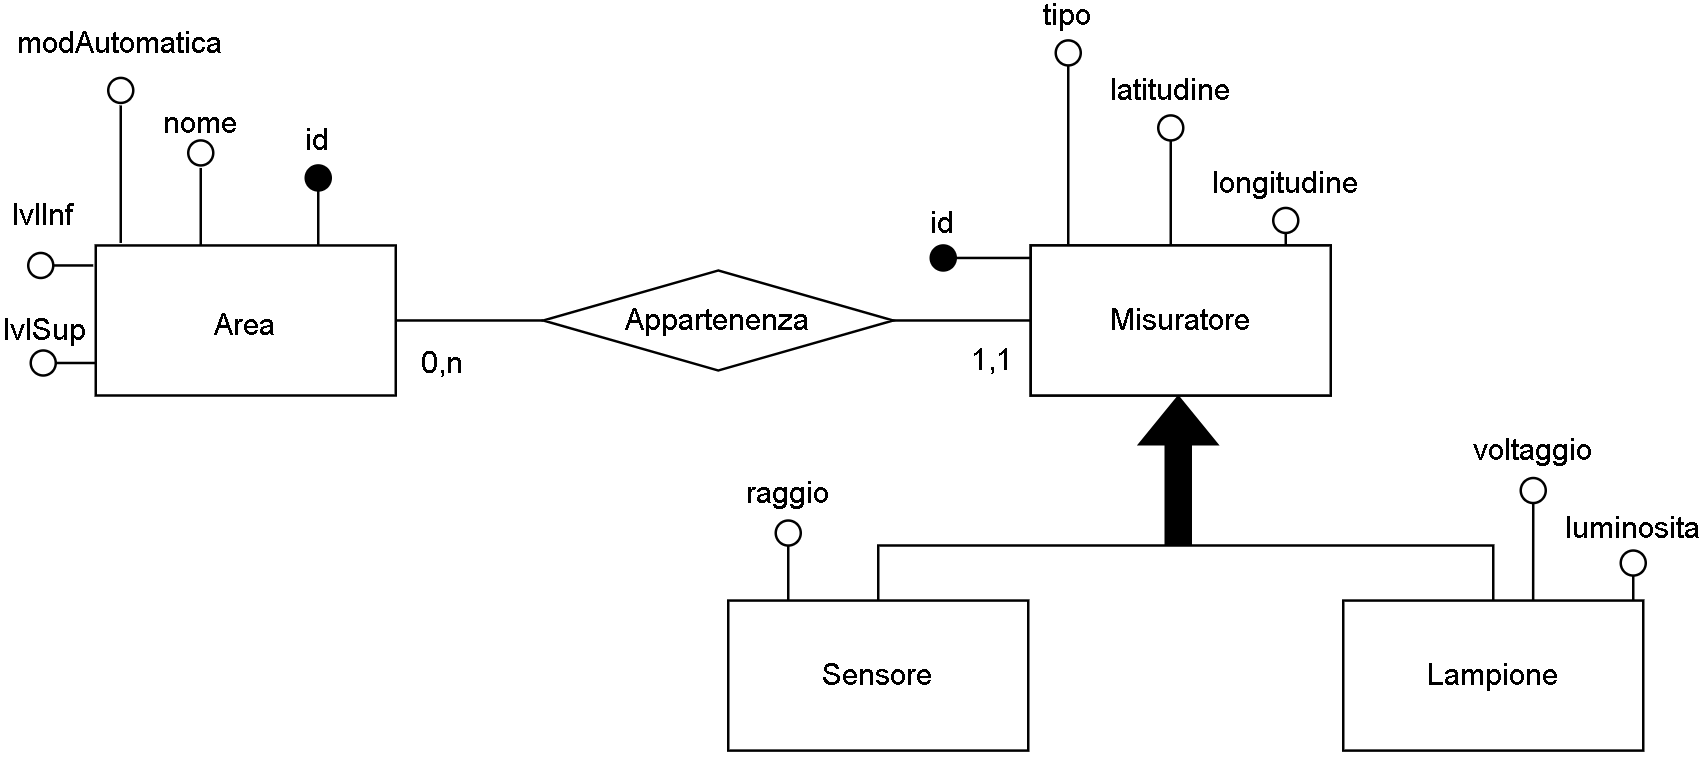
\includegraphics[width=12cm]{contenuti/specifica-basi-dati/img-sbd/anagrafica_concettuale.png}
\end{center}

\subsection{Progettazione logica}
